 \chapter{Plagiarism Report}
% We declare that the work presented in this project report is our original work. We acknowledge that copying someone else’s work or part of it is wrong. We have checked its plagiarism using online plagiarism checker and ensured that it is having more than 80\% originality.

% All sources used in this work have been correctly referenced, using proposer referencing. The work does not contain any sections that can be regarded as either a copy/cut-and-paste technique, as a mere translation, or as 'mono-phrasing’ (work taken from a single source). I realize that a design research argument has to be constructed, and declare that my text is a reflection of the integration of relevant sources. 
% \par
% Date : \dots \dots
% \par
% 	\vspace{0.008cm}
% 	\noindent
% 		\begin{tabular}{lcr}
% 		\\
% 		\bfseries  Avinash Maurya & \hspace{1.5cm} \textbf{Sneha Shukla} & \bfseries \hspace{2.5cm}  Utkarsh Tripathi\\
% 			Roll no. 2004331021 & \hspace{1.5cm}Roll no. 2004331049  &
%    Roll no. 2004331054
% 		\end{tabular}
%   \newpage
% \section*{\centering{\large \color{blue} Plagiarism Report }}

\begin{figure}[h]
	\centering 
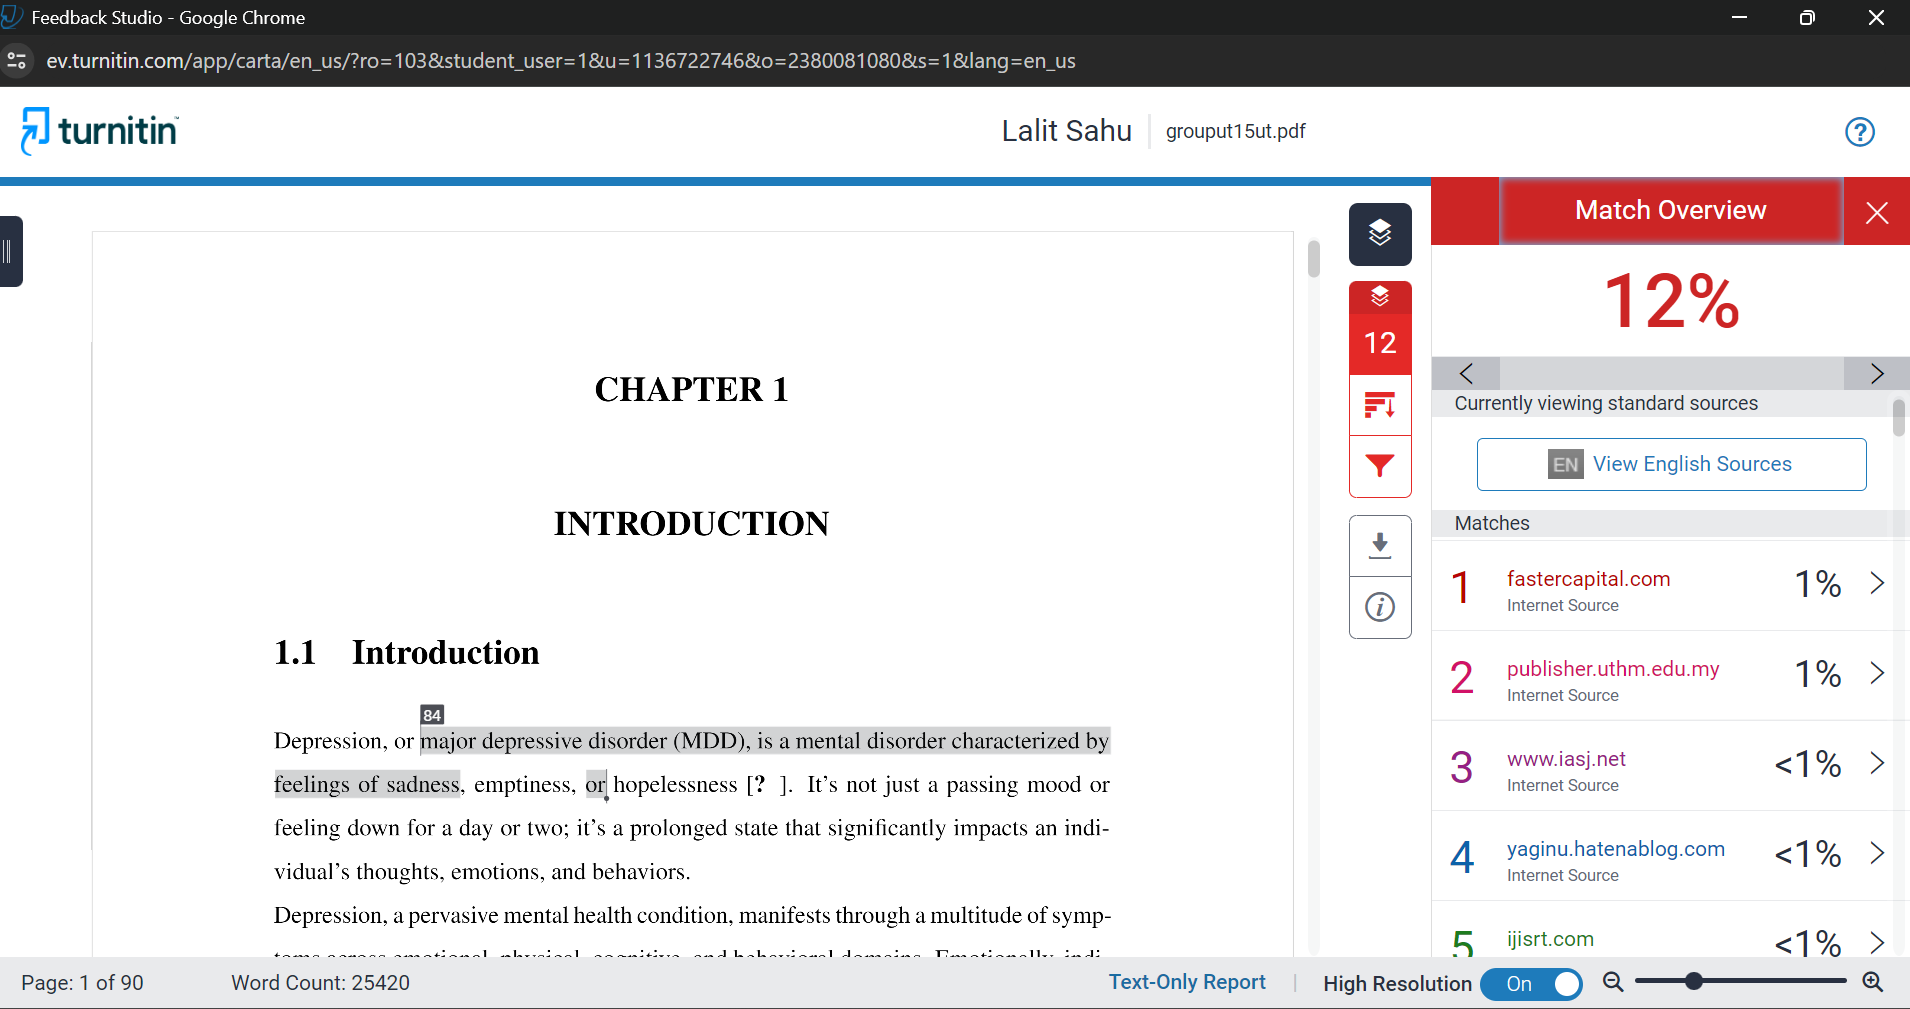
\includegraphics[width=\textwidth]{D_appx/plag1.png}
\end{figure}
\clearpage
\foreach \x in {1,2,...,5}
{
\clearpage
\begin{figure}
	\centering 
\includegraphics[width=\textwidth,page=\x]{D_appx/plagpdf.pdf}
\end{figure}
}
